\documentclass[11pt,a4paper]{article}
\usepackage[utf8]{inputenc}
\usepackage{float,graphicx,amsfonts,amsmath,amssymb,authblk,graphicx,longtable,booktabs,fullpage}
\usepackage{wrapfig}
\graphicspath{ {../img/} }
\usepackage[colorlinks = true,
            linkcolor = black,
            urlcolor  = blue,
            citecolor = blue,
            anchorcolor = blue]{hyperref}

% \title{Pendolo composto}

\title{%
  Pendolo composto \\
  \large Relazione: Esame di Laboratorio di Fisica 1}
    

\author[1]{Dennis Angemi}%
\affil[1]{Dipartimento di Fisica e Astronomia ``Ettore Majorana'' - Università degli Studi di Catania}%

\date{5 settembre 2022}

\begin{document}

\maketitle

\begin{abstract}
    È stato determinato il valore dell'accelerazione gravitazionale $g$ misurando il periodo di oscillazione di un pendolo fisico. Il valore ottenuto non risulta essere accurato tuttavia è possibile ritenerlo consistente con il valore teorico.
\end{abstract}

\section{Introduzione e cenni teorici}

Si definisce pendolo fisico o composto ogni corpo in grado di oscillare in un piano verticale attorno ad un asse orizzontale non passante per il centro di massa, per azione del suo peso.
\\
Per il teorema del momento angolare e per le definizioni di accelerazione angolare $\alpha$ e momento $M$ di una forza valgono le seguenti relazioni
\begin{equation}
    \begin{cases}
        \frac{dL}{dt} = I \alpha = I \frac{d^2 \theta}{dt^2} \\
        \frac{dL}{dt} = M = - mgd \sin \theta
    \end{cases} \Longrightarrow
    I \frac{d^2 \theta}{dt^2} = - mgd \sin \theta
\end{equation}
\\
da cui si conclude che
\begin{equation}
    \frac{d^2 \theta}{dt^2} + \frac{mgd}{I} \sin \theta = 0
\end{equation}
\begin{wrapfigure}{r}{0.5\textwidth}
  \begin{center}
    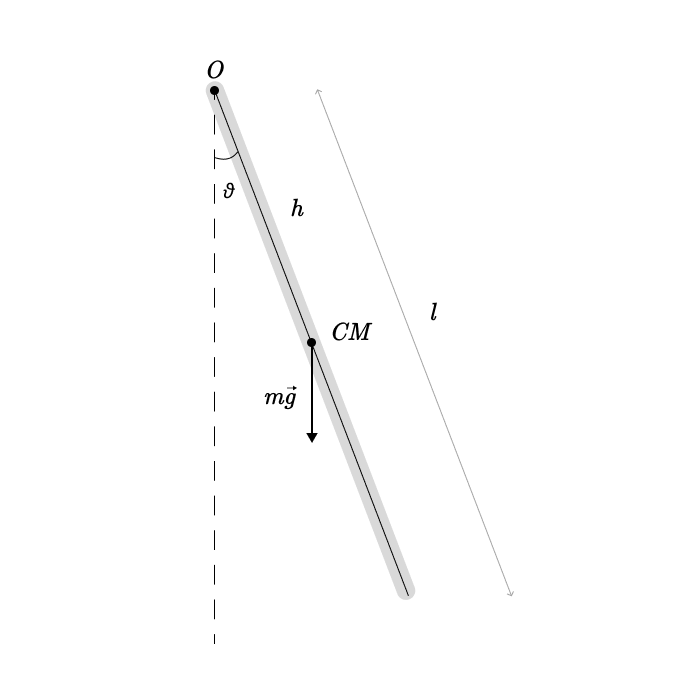
\includegraphics[width=0.48\textwidth]{img/pendolo.png}
  \end{center}
  \label{fig:pendolo}
  \caption{Diagramma delle forze}
\end{wrapfigure}
in cui:
\begin{itemize}
    \item $\theta$ rappresenta l'ampiezza dell'oscillazione (ovvero l'ampiezza dell'angolo acuto che il pendolo forma con la verticale passante per il vincolo $O$);
    \item $I$ rappresenta il momento d'inerzia del cilindro vincolato di lunghezza $l$.
\end{itemize}
\\
Se l'ampiezza $\theta$ delle oscillazioni è piccola, in modo tale da poter sfruttare l'approssimazione $\sin \theta = \theta$ , è possibile ottenere l'equazione del moto armonico del pendolo fisico
\begin{equation}
    \frac{d^2 \theta}{dt^2} + \frac{mgd}{I} \theta = 0
\end{equation}
\\
la cui forma più generale è
\begin{equation}
    \frac{d^2 \theta}{dt^2} + \omega^2 \theta = 0
\end{equation}
\\
con $\omega$ che rappresenta la pulsazione. Dalle eq. (3) e (4) si conclude che
\begin{equation}
    \omega = \sqrt{\frac{mgd}{I}}.
\end{equation}
È possibile ottenere esplicitamente la funzione $T(h)$, che lega il periodo di un'oscillazione $T$ alla distanza $d$ dell'asse di rotazione dal centro di massa, sfruttando la definizione di pulsazione $\omega$:
\begin{equation}
    \begin{cases}
        \omega = \frac{2 \pi}{T} \\
        \omega = \sqrt{\frac{mgd}{I}}
    \end{cases} \Longrightarrow
    T = 2 \pi \sqrt{\frac{I}{mgd}}.
\end{equation}
\\
Essendo $I$ il momento di inerzia di un cilindro di massa $m$ e lunghezza $l$ che ruota attorno ad un asse posto ad una distanza $d$ rispetto al suo centro di massa $CM$ (Figura \ref{fig:pendolo}), dal teorema di Huygens-Steiner segue
\begin{equation}
    I = I_{CM} + md^2 = m \left( \frac{l^2}{12} +d^2 \right)
\end{equation}
che permette di riscrivere l'eq. (6) come di seguito
\begin{equation}
    T = \left ( \frac{2 \pi}{\sqrt{g}} \right ) \sqrt{\frac{l^2}{12d}+d}
\end{equation}
\\
e ottenere l'accelerazione gravitazionale $g$ la cui determinazione della miglior stima è l'obiettivo dell'esperienza in questione
\begin{equation}
    g = \left( \frac{2 \pi}{T} \right)^2 \frac{I}{md} = \left( \frac{2 \pi}{T} \right)^2 \left( \frac{1}{12} \frac{l^2}{d} + d \right).
    \label{eq:defg}
\end{equation}

\section{Apparato sperimentale}

\subsection{Descrizione apparato}
L'apparato sperimentale è costituito da un cilindro di lunghezza $l = (1 \pm 0.01) \; m$ vincolato ad un perno mobile che, oltre a consentire le oscillazioni del pendolo, permette allo sperimentatore di variare la distanza $d$ tra l'asse di rotazione e il centro di massa del cilindro.

\subsection{Strumenti di misura}

\begin{longtable}[]{@{}lllll@{}}
    \toprule
    Strumento & Sensibilità \tabularnewline
    \midrule
    \endhead
    Cronometro & 0.01 \; s \tabularnewline
    Metro & 1 \; cm \tabularnewline
    Sensore di prossimità TMD4906 & 0.05 \; s \tabularnewline
    \bottomrule
    \caption{Strumenti di misura}
    \label{tab:tool}
\end{longtable}


\subsection{Procedura di misura}
Si è proceduto alla misurazione degli intervalli di tempo $t$ impiegato dal pendolo a compiere mezza oscillazione mediante il sensore di prossimità TMD4906 di uno smartphone Samsung Galaxy S8 posizionato al di sotto del cilindro; nella fase di data collection è stato sfruttato il software Physics Toolbox Sensor Suite. 
Essendo possibile variare la distanza $d$, sono state individuate 13 configurazioni per ognuna delle quali sono state effettuate 100 misurazioni di $t$ .

\begin{longtable}[]{@{}lllll@{}}
    \toprule
    Configurazione & Lunghezza ($\pm 0.2 \; cm$) \tabularnewline
    \midrule
    \endhead
1 & 60 \tabularnewline
2 & 65 \tabularnewline
3 & 70 \tabularnewline
4 & 72 \tabularnewline
5 & 75 \tabularnewline
6 & 77 \tabularnewline
7 & 80 \tabularnewline
8 & 82 \tabularnewline
9 & 85 \tabularnewline
10 & 87 \tabularnewline
11 & 90 \tabularnewline
12 & 92 \tabularnewline
13 & 95 \tabularnewline
    \bottomrule
    \\
    \caption{Configurazioni}
    \label{tab:conf}
\end{longtable}
\\
Si noti che :
\begin{itemize}
    \item le misure della lunghezza del pendolo risultano poco precise per via della difficoltà riscontrata nell'interpolazione in fase di lettura: il cilindro è dotato di incisioni poste ad una distanza di 1 $cm$ l'una dall'altra;
    
    \item la lunghezza in Tabella \ref{tab:conf} non coincide con la distanza $d$ di cui sopra;
    
    \item È possibile consultare i dati relativi alle circa 1300 misure in Appendice A.
\end{itemize}


\section{Analisi dei dati e propagazione degli errori}
\subsection{Test del $\chi^2$}
Avendo effettuato 100 misurazione di $t$ per ogni configurazione, si è proceduto all'analisi della distribuzione dei valori osservati al fine di verificare se i risultati dell'esperimento sono governati dalla distribuzione limite normale attesa. Selezionando arbitrariamente la configurazione 6, si è proceduto alla determinazione della media $\bar{t}$ e della deviazione standard $\sigma_t$ come da eq. \ref{eq:mstd6}
\begin{equation}
    \bar{t} = \frac{1}{N} \sum_{i=1}^N t_i = 777.2 \; s \; \; \; \; \; \; \; \; \; \; \; \; \; \; \sigma_t = \sqrt{\frac{1}{N-1} \sum_{i=1}^N  (t_i - \bar{t})^2} = 2.1 \; s
    \label{eq:mstd6}
\end{equation}
e gli $N=100$ valori sono stati disposti in 4 intervalli le cui caratteristiche sono riassunte in Tabella \ref{tab:conf6}
\begin{longtable}[]{@{}lllll@{}}
    \toprule
    intervallo $k$ & estremi & probabilità $P_k$ & numero atteso $E_k$ & numero osservato $O_k$\tabularnewline
    \midrule
    \endhead
    1 & $t < \bar{t} - \sigma$ & 0.16 & 16.16 & 21 \tabularnewline
    2 & $\bar{t} - \sigma< t < \bar{t}$ & 0.34 & 34.34 & 37 \tabularnewline
    3 & $\bar{t} < t < \bar{t} + \sigma$ & 0.34 & 34.34 & 30 \tabularnewline
    4 & $t > \bar{t} + \sigma$ & 0.16 & 16.16 & 13 \tabularnewline
    \bottomrule
    \label{tab:conf6}
    \\
    \caption{Configurazione 6}
\end{longtable}

Dai dati in Tabella \ref{tab:conf6} è stato possibile calcolare 
\begin{equation}
    \chi^2 = \sum_{k=1}^n \frac{(O_k - E_k)^2}{E_k} = 2.8
\end{equation}
con
\begin{itemize}
    \item $O_k$ numeri osservati nell'intervallo $k$
    \item $E_k$ numeri attesi nell'intervallo $k$.
\end{itemize}
Dal momento che il numero di intervalli $k$ è pari a 4 e che i vincoli della distribuzione gaussiana sono pari a 3, si conclude che i gradi di liberà $d=1$ e di conseguenza il valore $\chi^2 = 2.8$ coincide con il valore del chi-quadro ridotto $\tilde{\chi}^2$ . Non essendo verificata la condizione $\tilde{\chi}^2 >> 1$ ed essendo $\chi^2$ dell'ordine di $n$, è ragionevole supporre che le misure $t_i$ siano governate dalla distribuzione attesa: la distribuzione normale.
\begin{figure}[H]
    \centering
    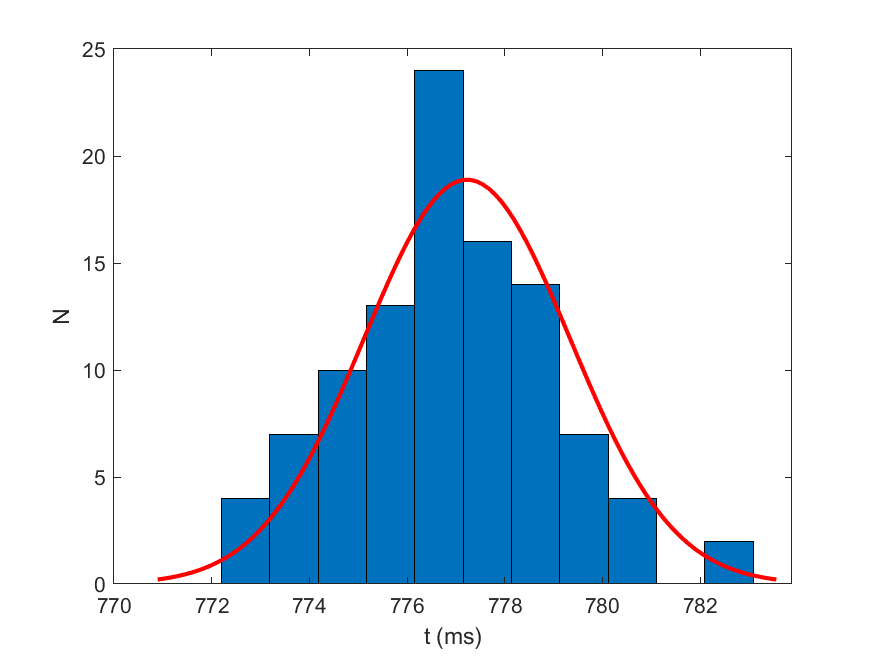
\includegraphics[scale = .6]{img/chi.png}
    \caption{Distribuzione delle misure $t_i$ della configurazione 6}
    \label{fig:my_label}
\end{figure}

\subsection{Analisi statistica}
Per ogni configurazione $j$ (con $j = 1, 2, ..., 13$) si è proceduto al calcolo della media dei periodi $T_i$ e della deviazione standard $\sigma_T$
\begin{equation}
    \sigma_T = \sqrt{\frac{1}{N-1} \sum_{i=1}^N  (T_i - \bar{T})^2}.
\end{equation}
È stata determinata inoltre la distanza $d$ sottraendo 50 cm alla lunghezza riportata in Tabella \ref{tab:conf}

\begin{longtable}[]{@{}lllll@{}}
    \toprule
    Configuration j & $\bar{T} (s)$ & $\sigma_T$ & d (m) \tabularnewline
    \midrule
    \endhead
1 & 1.995 & 0.004 & 0.1 \tabularnewline
2 & 1.74 & 0.02 & 0.15 \tabularnewline
3 & 1.65 & 0.02 & 0.2 \tabularnewline
4 & 1.62 & 0.02 & 0.22 \tabularnewline
5 & 1.56 & 0.02 & 0.25 \tabularnewline
6 & 1.555 & 0.004 & 0.27 \tabularnewline
7 & 1.53 & 0.02 & 0.3 \tabularnewline
8 & 1.57 & 0.02 & 0.32 \tabularnewline
9 & 1.54 & 0.02 & 0.35 \tabularnewline
10 & 1.59 & 0.02 & 0.37 \tabularnewline
11 & 1.596 & 0.004 & 0.4 \tabularnewline
12 & 1.60 & 0.02 & 0.42 \tabularnewline
13 & 1.636 & 0.009 & 0.45 \tabularnewline
    \bottomrule
    \\
    \caption{Periodi $\bar{T}$ in funzione di $d$}
    \label{tab:td}
\end{longtable}
Dalla Figura \ref{fig:teocu}, rappresentante i dati in Tabella \ref{tab:td}, è possibile osservare come soltanto due valori osservati siano perfettamente in accordo con la curva teorica descritta dalla funzione
\begin{equation}
    T(d) = 2 \pi \sqrt{\frac{1}{gd} \left( \frac{l^2}{12} + d^2 \right)}.
    \label{eq:teocu}
\end{equation}
\begin{figure}
    \centering
    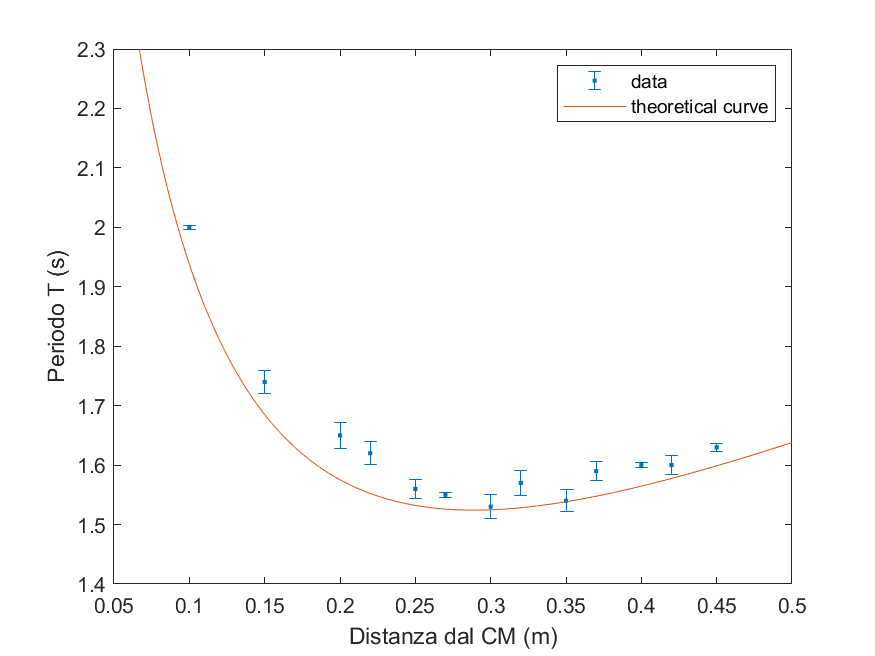
\includegraphics[scale=0.8]{img/plot2.png}
    \caption{Periodo $T$ in funzione della distanza $d$}
    \label{fig:teocu}
\end{figure}
\\
Linearizzando l'eq. \ref{eq:teocu} si ottiene la seguente espressione per $T(d)$

\begin{equation}
    T = \left ( \frac{2 \pi}{\sqrt{g}} \right ) \sqrt{\frac{l^2}{12d}+d}
\end{equation}
\\
in cui il fattore $\frac{2 \pi}{\sqrt{g}}$ rappresenta il coefficiente angolare della retta che meglio approssima i dati sperimentali. Si applica quindi il metodo dei minimi quadrati considerando una generica funzione $y = A + Bx$ ed effettuando le seguenti posizioni
\begin{equation}
    y = \bar{T} \; \; \; \; \; \; \; \; \; \; \; \; \; \; \; \; \; \; x = \sqrt{\frac{l^2}{12d}+d}.
\end{equation}
È possibile stimare i parametri $A$ e $B$ applicando il metodo dei minimi quadrati come di seguito
\begin{equation}
    A = \frac{\sum x^2 \sum y - \sum x \sum xy}{\Delta} = 00.9; \; \;  \; \; \; \;\; \; \; \; \; \; \; B = \frac{N\sum xy - \sum x \sum y}{\Delta} = 2.2
\end{equation}
\\
con
\begin{equation}
    \Delta = N \sum x^2 - \left( \sum x \right )^2.
\end{equation}
\\
Le incertezze nella misura di y e nei parametri A e B risultano essere rispettivamente
\begin{equation}
    \sigma_y = \sqrt{\frac{1}{N-2} \sum_i (y_i - A - Bx_i)^2} = 0.02
\end{equation}
\\
\begin{equation}
    \sigma_A = \sigma_y \sqrt{\frac{\sum x^2}{\Delta}}; \; \; \; \; \; \; \; \; \; \; \; \; \; \; \sigma_B = \sigma_y \sqrt{\frac{N}{\Delta}}.
\end{equation}
\\
Si conclude dunque che
\begin{equation}
    A = -0.09 \pm 0.08,
\end{equation}
\begin{equation}
   B = 2.2 \pm 0.1
\end{equation}
\\
pertanto la retta di best fit assume la forma
\begin{equation}
    y = -0.09 + 2.2x
\end{equation}
\begin{figure}[H]
    \centering
    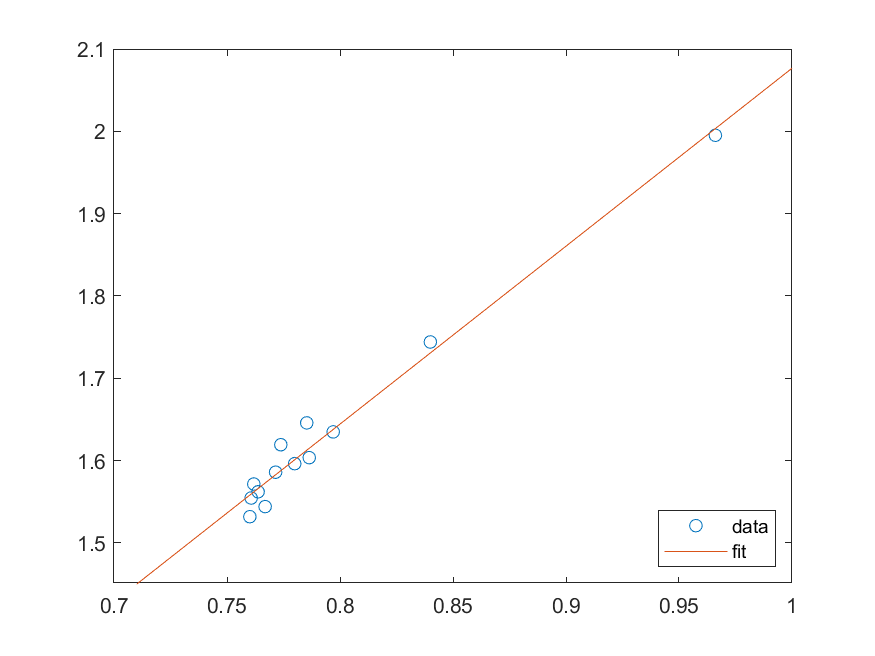
\includegraphics[scale = .7]{img/plot4.png}
    \caption{Best fit}
    \label{fig:bestfit}
\end{figure}
\\
Al fine di valutare la correlazione delle grandezze $y$ e $x$, si procede al calcolo del coefficiente di correlazione lineare
\\
\begin{equation}
    r = \frac{\sum (x_i - \bar{x})(y_i - \bar{y})}{\sqrt{\sum (x_i - \bar{x})^2 \sum (y_i - \bar{y})^2}} = 0.99
\end{equation}
\\
dal cui valore è possibile comprendere come i punti ($x_i,y_i$) si adattino praticamente in modo perfetto alla retta $y$. Essendo $B$ pari al coefficiente angolare della retta $y$ è possibile stimare il valore dell'accelerazione gravitazionale $g$ come di seguito
\begin{wrapfigure}{r}{0.5\textwidth}
  \begin{center}
    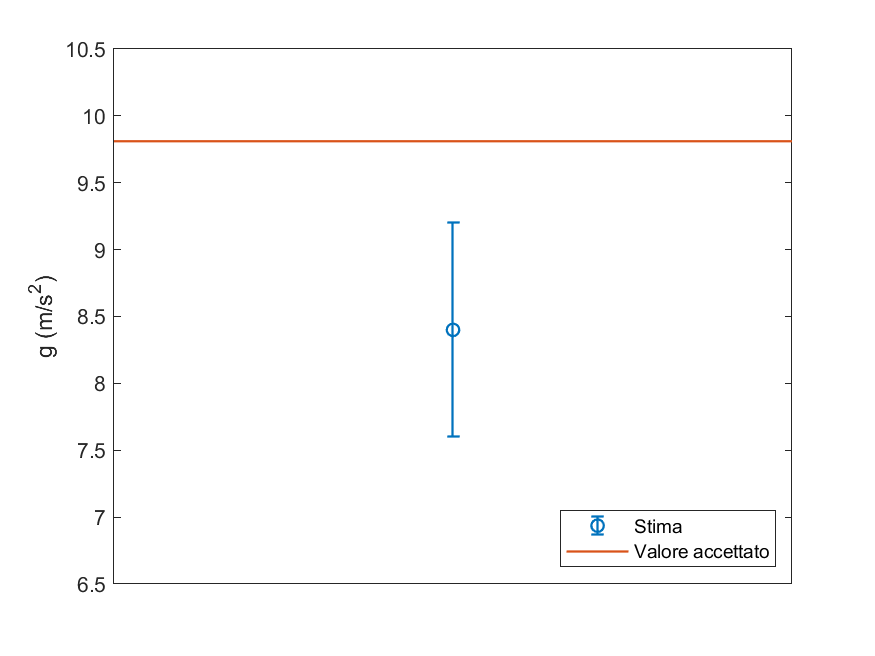
\includegraphics[width=0.48\textwidth]{img/gplot1.png}
  \end{center}
  \label{fig:gbest}
  %\caption{$g_{best}$ e valore accettato }
\end{wrapfigure}
\begin{equation}
    B = \frac{2 \pi}{\sqrt{g}} \Longleftrightarrow g = \left( \frac{2 \pi}{B} \right )^2 = 8.4 \; m/s^2.
\end{equation}
L'incertezza su $g$ sarà data dalla propagazione degli errori
\begin{equation}
    \sigma_g = \left | \frac{\partial g}{\partial B} \right | \sigma_B = \frac{8 \pi^2}{B^3} \sigma_B = 0.8 \; m/s^2.
\end{equation}
Si conclude quindi che 
\begin{equation}
    g_{best} = 8.4 \pm 0.8 \; m/s^2
\end{equation}
un valore che differisce dal valore accettato (9.8 $m/s^2$) di 1.75 $\sigma_g$.
\\
\\
Oltre alla determinazione della miglior stima dell'accelerazione gravitazionale $g_{best}$ applicando il metodo dei minimi quadrati, si è ritenuto opportuno procedere ad un'ulteriore stima di $g$ (effettuata per ogni configurazione $j$) la cui determinazione si avvale dell'eq. \ref{eq:defg}. I risultati del procedimento descritto (dotati della loro deviazione standard) sono rappresentati in Figura \ref{fig:gmconf} e riportati nel dettaglio in Tabella \ref{tab:gm}.
\begin{figure}[H]
    \centering
    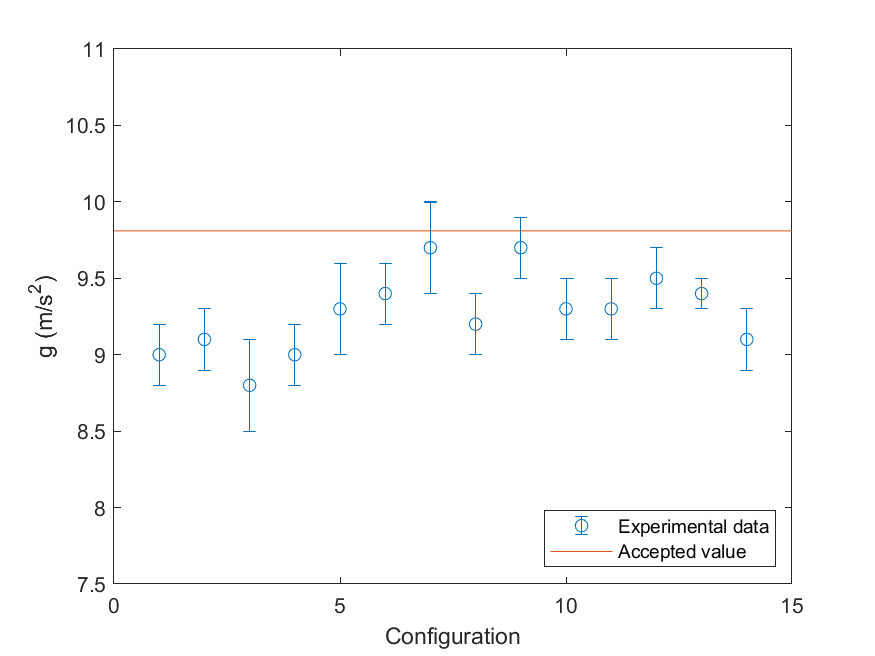
\includegraphics[scale=0.6]{img/plot5.png}
    \caption{$\bar{g}$ in funzione delle 13 configurazioni}
    \label{fig:gmconf}
\end{figure}


\begin{longtable}[]{@{}lllll@{}}
    \toprule
    Configurazione $j$ & $\bar{g}_j$ & $\sigma_g$ \tabularnewline
    \midrule
    \endhead
1 & 9.26 & 0.04 \tabularnewline
2 & 9.2 & 0.2 \tabularnewline
3 & 9.0 & 0.2 \tabularnewline
4 & 9.0 & 0.2 \tabularnewline
5 & 9.4 & 0.2 \tabularnewline
6 & 9.45 & 0.05 \tabularnewline
7 & 9.7 & 0.3 \tabularnewline
8 & 9.3 & 0.2 \tabularnewline
9 & 9.7 & 0.2 \tabularnewline
10 & 9.4 & 0.2 \tabularnewline
11 & 9.43 & 0.05 \tabularnewline
12 & 9.5 & 0.12 \tabularnewline
13 & 9.4 & 0.1 \tabularnewline
    \bottomrule
    \\
    \caption{Valori di $\bar{g}$ in funzione delle 13 configurazioni}
    \label{tab:gm}
\end{longtable}

Il valore medio $\bar{g}$ delle misure riportate in Tabella \ref{tab:gm} è $\bar{g} = 9.4 \pm 0.2 \; m/s^2$.

\section{Risultati e conclusioni}
La migliore stima di $g_{best}$, ottenuta a seguito dell'applicazione del metodo dei minimi quadrati, e il valore $\bar{g}$ ottenuto mediando risultano essere rispettivamente
\begin{equation}
    g_{best} = 8.4 \pm 0.8 \; m/s^2 \; \; \; \; \; \; \; \; \; \bar{g} = 9.4 \pm 0.2 \; m/s^2.
    \label{eq:concl}
\end{equation}
\begin{figure}[H]
    \centering
    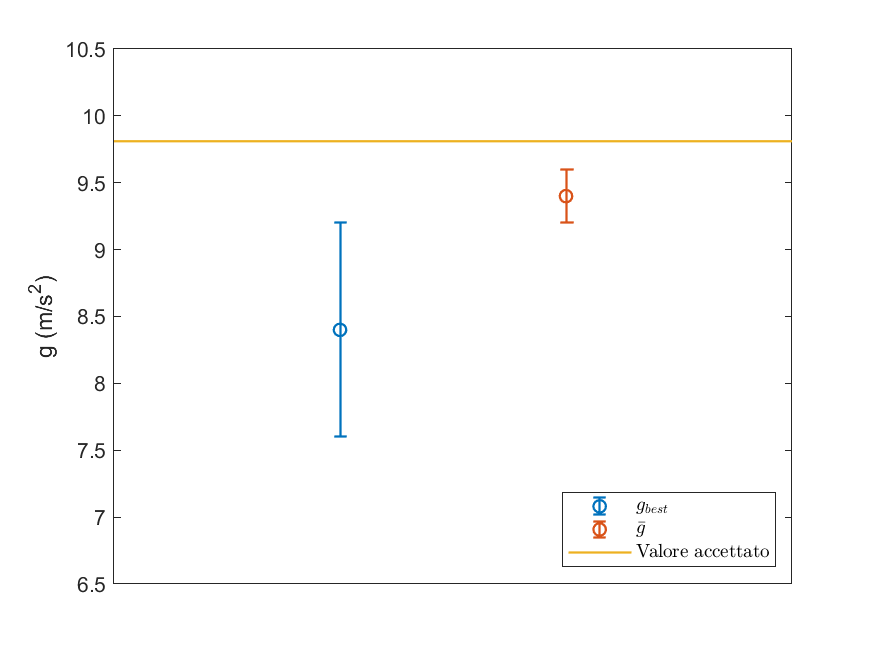
\includegraphics[scale=0.7]{img/gplot2.png}
    \caption{Gli intervalli di $g_{best}$ e $\bar{g}$ a confronto}
    \label{fig:gconcl}
\end{figure}
\\
Gli intervalli probabili di $g_{best}$ e $\bar{g}$ raffigurati in Figura \ref{fig:gconcl} si sovrappongono pertanto risultano essere in buon accordo. Entrambi i valori di $g_{best}$ e $\bar{g}$ non differiscono dal valore accettato di 9.8 $m/s^2$ per più di 2 $\sigma$ e da ciò è ragionevole affermare che, nonostante l'esperimento non sia conclusivo e i risultati ottenuti siano dotati di una scarsa accuratezza, essi risultano comunque essere consistenti con il valore accettato. In particolare $g_{best}$ differisce dal valore noto di 1.75 $\sigma_g$ e $\bar{g}$ differisce dal valore noto di 2 $\sigma_\bar{g}$.

\section{Additional notes}

\subsection{Data Availability}
The data that support the findings of this study are openly available in \href{https://github.com/dennisangemi/lab1-exam/tree/main/data}{dennisangemi/lab1-exam GitHub Repository} at \href{https://github.com/dennisangemi/lab1-exam}{https://github.com/dennisangemi/lab1-exam/tree/main/data} under \href{https://creativecommons.org/licenses/by/4.0/}{CC-BY 4.0 license}.

\subsection{Code Availability}
The MATLAB code written to get the findings of this study is openly available in \href{https://github.com/dennisangemi/lab1-exam/tree/main/scripts}{dennisangemi/lab1-exam GitHub Repository} at \href{https://github.com/dennisangemi/lab1-exam/tree/main/scripts}{https://github.com/dennisangemi/lab1-exam/tree/main/scripts}


\subsection{Software used}
\begin{itemize}
    \item \textbf{MATLAB}: Data Analysis
    \item \textbf{Physics Toolbox Sensor Suite}: Data Collection
    \item \textbf{GitHub}: Resource sharing
    \item \textbf{Figma}: Images designing
\end{itemize}

\section{Bibliography}
\begin{itemize}
    \item Taylor,~ J. (1999).~\emph{Introduzione all'analisi degli errori: Lo
  studio delle incertezze nelle misure fisiche.~}Zanichelli
    \item Bevington, P. (2002).~\emph{Data Reduction and Error Analysis for the Physical Sciences.~} McGraw-Hill Education ~
    \item Malthe-Sørenssen, A. (2015). \emph{Elementary Mechanics Using Matlab: A Modern Course Combining Analytical and Numerical Techniques}. Springer
    \item Mazzoldi, P., Nigro, M., Voci, C. (2001). \emph{Fisica. Meccanica, termodinamica (Vol. 1)}. Edises
\end{itemize}

\section{Appendice A}
\subsection{Tabella 1}
\begin{longtable}[]{@{}lllll@{}}
    \toprule
    Configuration & Event & Time (ms) \tabularnewline
    \midrule
    \endhead
1 & 1 & 1002 \tabularnewline
1 & 2 & 995 \tabularnewline
1 & 3 & 998 \tabularnewline
1 & 4 & 1000 \tabularnewline
1 & 5 & 996 \tabularnewline
1 & 6 & 998 \tabularnewline
1 & 7 & 997 \tabularnewline
1 & 8 & 997 \tabularnewline
1 & 9 & 996 \tabularnewline
1 & 10 & 1000 \tabularnewline
1 & 11 & 995 \tabularnewline
1 & 12 & 997 \tabularnewline
1 & 13 & 997 \tabularnewline
1 & 14 & 999 \tabularnewline
1 & 15 & 995 \tabularnewline
1 & 16 & 998 \tabularnewline
1 & 17 & 998 \tabularnewline
1 & 18 & 997 \tabularnewline
1 & 19 & 1000 \tabularnewline
1 & 20 & 993 \tabularnewline
1 & 21 & 999 \tabularnewline
1 & 22 & 997 \tabularnewline
1 & 23 & 998 \tabularnewline
1 & 24 & 998 \tabularnewline
1 & 25 & 997 \tabularnewline
1 & 26 & 995 \tabularnewline
1 & 27 & 998 \tabularnewline
1 & 28 & 1001 \tabularnewline
1 & 29 & 997 \tabularnewline
1 & 30 & 998 \tabularnewline
1 & 31 & 998 \tabularnewline
1 & 32 & 997 \tabularnewline
1 & 33 & 998 \tabularnewline
1 & 34 & 1001 \tabularnewline
1 & 35 & 998 \tabularnewline
1 & 36 & 998 \tabularnewline
1 & 37 & 998 \tabularnewline
1 & 38 & 994 \tabularnewline
1 & 39 & 998 \tabularnewline
2 & 1 & 883 \tabularnewline
2 & 2 & 887 \tabularnewline
2 & 3 & 860 \tabularnewline
2 & 4 & 856 \tabularnewline
2 & 5 & 876 \tabularnewline
2 & 6 & 854 \tabularnewline
2 & 7 & 857 \tabularnewline
2 & 8 & 874 \tabularnewline
2 & 9 & 872 \tabularnewline
2 & 10 & 878 \tabularnewline
2 & 11 & 878 \tabularnewline
2 & 12 & 877 \tabularnewline
2 & 13 & 856 \tabularnewline
2 & 14 & 874 \tabularnewline
2 & 15 & 862 \tabularnewline
2 & 16 & 858 \tabularnewline
2 & 17 & 872 \tabularnewline
2 & 18 & 860 \tabularnewline
2 & 19 & 878 \tabularnewline
2 & 20 & 876 \tabularnewline
2 & 21 & 876 \tabularnewline
2 & 22 & 880 \tabularnewline
2 & 23 & 881 \tabularnewline
2 & 24 & 882 \tabularnewline
2 & 25 & 876 \tabularnewline
2 & 26 & 855 \tabularnewline
2 & 27 & 862 \tabularnewline
2 & 28 & 875 \tabularnewline
2 & 29 & 877 \tabularnewline
2 & 30 & 873 \tabularnewline
2 & 31 & 895 \tabularnewline
2 & 32 & 858 \tabularnewline
2 & 33 & 876 \tabularnewline
2 & 34 & 877 \tabularnewline
2 & 35 & 879 \tabularnewline
2 & 36 & 876 \tabularnewline
2 & 37 & 863 \tabularnewline
2 & 38 & 874 \tabularnewline
2 & 39 & 889 \tabularnewline
2 & 40 & 881 \tabularnewline
2 & 41 & 877 \tabularnewline
2 & 42 & 875 \tabularnewline
2 & 43 & 878 \tabularnewline
2 & 44 & 876 \tabularnewline
2 & 45 & 874 \tabularnewline
2 & 46 & 875 \tabularnewline
2 & 47 & 875 \tabularnewline
2 & 48 & 876 \tabularnewline
2 & 49 & 878 \tabularnewline
2 & 50 & 877 \tabularnewline
2 & 51 & 870 \tabularnewline
2 & 52 & 875 \tabularnewline
2 & 53 & 885 \tabularnewline
2 & 54 & 875 \tabularnewline
2 & 55 & 862 \tabularnewline
2 & 56 & 857 \tabularnewline
2 & 57 & 861 \tabularnewline
2 & 58 & 857 \tabularnewline
2 & 59 & 855 \tabularnewline
2 & 60 & 857 \tabularnewline
2 & 61 & 875 \tabularnewline
2 & 62 & 873 \tabularnewline
2 & 63 & 874 \tabularnewline
2 & 64 & 880 \tabularnewline
2 & 65 & 888 \tabularnewline
2 & 66 & 875 \tabularnewline
2 & 67 & 860 \tabularnewline
2 & 68 & 874 \tabularnewline
2 & 69 & 875 \tabularnewline
2 & 70 & 876 \tabularnewline
2 & 71 & 875 \tabularnewline
2 & 72 & 876 \tabularnewline
2 & 73 & 861 \tabularnewline
2 & 74 & 876 \tabularnewline
2 & 75 & 874 \tabularnewline
2 & 76 & 854 \tabularnewline
2 & 77 & 879 \tabularnewline
2 & 78 & 853 \tabularnewline
2 & 79 & 876 \tabularnewline
2 & 80 & 874 \tabularnewline
2 & 81 & 884 \tabularnewline
2 & 82 & 856 \tabularnewline
2 & 83 & 882 \tabularnewline
3 & 1 & 818 \tabularnewline
3 & 2 & 821 \tabularnewline
3 & 3 & 818 \tabularnewline
3 & 4 & 819 \tabularnewline
3 & 5 & 817 \tabularnewline
3 & 6 & 837 \tabularnewline
3 & 7 & 818 \tabularnewline
3 & 8 & 857 \tabularnewline
3 & 9 & 820 \tabularnewline
3 & 10 & 819 \tabularnewline
3 & 11 & 860 \tabularnewline
3 & 12 & 818 \tabularnewline
3 & 13 & 818 \tabularnewline
3 & 14 & 817 \tabularnewline
3 & 15 & 817 \tabularnewline
3 & 16 & 817 \tabularnewline
3 & 17 & 821 \tabularnewline
3 & 18 & 820 \tabularnewline
3 & 19 & 820 \tabularnewline
3 & 20 & 818 \tabularnewline
3 & 21 & 840 \tabularnewline
3 & 22 & 837 \tabularnewline
3 & 23 & 816 \tabularnewline
3 & 24 & 814 \tabularnewline
3 & 25 & 836 \tabularnewline
3 & 26 & 817 \tabularnewline
3 & 27 & 814 \tabularnewline
3 & 28 & 858 \tabularnewline
3 & 29 & 817 \tabularnewline
3 & 30 & 832 \tabularnewline
3 & 31 & 819 \tabularnewline
3 & 32 & 820 \tabularnewline
3 & 33 & 818 \tabularnewline
3 & 34 & 841 \tabularnewline
3 & 35 & 819 \tabularnewline
3 & 36 & 816 \tabularnewline
3 & 37 & 821 \tabularnewline
3 & 38 & 879 \tabularnewline
3 & 39 & 815 \tabularnewline
3 & 40 & 819 \tabularnewline
3 & 41 & 820 \tabularnewline
3 & 42 & 817 \tabularnewline
3 & 43 & 835 \tabularnewline
3 & 44 & 839 \tabularnewline
3 & 45 & 834 \tabularnewline
3 & 46 & 837 \tabularnewline
3 & 47 & 815 \tabularnewline
3 & 48 & 818 \tabularnewline
3 & 49 & 821 \tabularnewline
3 & 50 & 817 \tabularnewline
3 & 51 & 857 \tabularnewline
3 & 52 & 815 \tabularnewline
3 & 53 & 816 \tabularnewline
3 & 54 & 817 \tabularnewline
3 & 55 & 814 \tabularnewline
3 & 56 & 835 \tabularnewline
3 & 57 & 799 \tabularnewline
3 & 58 & 821 \tabularnewline
3 & 59 & 819 \tabularnewline
3 & 60 & 818 \tabularnewline
3 & 61 & 815 \tabularnewline
3 & 62 & 841 \tabularnewline
3 & 63 & 817 \tabularnewline
3 & 64 & 838 \tabularnewline
3 & 65 & 815 \tabularnewline
3 & 66 & 820 \tabularnewline
3 & 67 & 818 \tabularnewline
3 & 68 & 818 \tabularnewline
3 & 69 & 816 \tabularnewline
3 & 70 & 818 \tabularnewline
3 & 71 & 819 \tabularnewline
3 & 72 & 836 \tabularnewline
3 & 73 & 819 \tabularnewline
3 & 74 & 818 \tabularnewline
3 & 75 & 816 \tabularnewline
3 & 76 & 816 \tabularnewline
3 & 77 & 818 \tabularnewline
3 & 78 & 818 \tabularnewline
3 & 79 & 820 \tabularnewline
3 & 80 & 816 \tabularnewline
3 & 81 & 821 \tabularnewline
3 & 82 & 821 \tabularnewline
3 & 83 & 818 \tabularnewline
4 & 1 & 820 \tabularnewline
4 & 2 & 814 \tabularnewline
4 & 3 & 820 \tabularnewline
4 & 4 & 798 \tabularnewline
4 & 5 & 800 \tabularnewline
4 & 6 & 816 \tabularnewline
4 & 7 & 814 \tabularnewline
4 & 8 & 799 \tabularnewline
4 & 9 & 797 \tabularnewline
4 & 10 & 817 \tabularnewline
4 & 11 & 799 \tabularnewline
4 & 12 & 800 \tabularnewline
4 & 13 & 816 \tabularnewline
4 & 14 & 817 \tabularnewline
4 & 15 & 819 \tabularnewline
4 & 16 & 797 \tabularnewline
4 & 17 & 818 \tabularnewline
4 & 18 & 818 \tabularnewline
4 & 19 & 798 \tabularnewline
4 & 20 & 813 \tabularnewline
4 & 21 & 793 \tabularnewline
4 & 22 & 795 \tabularnewline
4 & 23 & 798 \tabularnewline
4 & 24 & 814 \tabularnewline
4 & 25 & 797 \tabularnewline
4 & 26 & 800 \tabularnewline
4 & 27 & 814 \tabularnewline
4 & 28 & 816 \tabularnewline
4 & 29 & 817 \tabularnewline
4 & 30 & 818 \tabularnewline
4 & 31 & 814 \tabularnewline
4 & 32 & 817 \tabularnewline
4 & 33 & 816 \tabularnewline
4 & 34 & 799 \tabularnewline
4 & 35 & 798 \tabularnewline
4 & 36 & 797 \tabularnewline
4 & 37 & 818 \tabularnewline
4 & 38 & 793 \tabularnewline
4 & 39 & 798 \tabularnewline
4 & 40 & 817 \tabularnewline
4 & 41 & 797 \tabularnewline
4 & 42 & 817 \tabularnewline
4 & 43 & 818 \tabularnewline
4 & 44 & 817 \tabularnewline
4 & 45 & 800 \tabularnewline
4 & 46 & 794 \tabularnewline
4 & 47 & 796 \tabularnewline
4 & 48 & 817 \tabularnewline
4 & 49 & 817 \tabularnewline
4 & 50 & 821 \tabularnewline
4 & 51 & 797 \tabularnewline
4 & 52 & 817 \tabularnewline
4 & 53 & 818 \tabularnewline
4 & 54 & 816 \tabularnewline
4 & 55 & 817 \tabularnewline
4 & 56 & 816 \tabularnewline
4 & 57 & 817 \tabularnewline
4 & 58 & 815 \tabularnewline
4 & 59 & 815 \tabularnewline
4 & 60 & 817 \tabularnewline
4 & 61 & 818 \tabularnewline
4 & 62 & 821 \tabularnewline
4 & 63 & 816 \tabularnewline
4 & 64 & 814 \tabularnewline
4 & 65 & 800 \tabularnewline
4 & 66 & 818 \tabularnewline
4 & 67 & 815 \tabularnewline
4 & 68 & 797 \tabularnewline
4 & 69 & 817 \tabularnewline
4 & 70 & 797 \tabularnewline
4 & 71 & 820 \tabularnewline
4 & 72 & 817 \tabularnewline
4 & 73 & 799 \tabularnewline
4 & 74 & 817 \tabularnewline
4 & 75 & 818 \tabularnewline
4 & 76 & 797 \tabularnewline
4 & 77 & 818 \tabularnewline
4 & 78 & 816 \tabularnewline
4 & 79 & 798 \tabularnewline
4 & 80 & 815 \tabularnewline
4 & 81 & 816 \tabularnewline
4 & 82 & 794 \tabularnewline
4 & 83 & 818 \tabularnewline
4 & 84 & 797 \tabularnewline
4 & 85 & 816 \tabularnewline
4 & 86 & 799 \tabularnewline
5 & 1 & 778 \tabularnewline
5 & 2 & 778 \tabularnewline
5 & 3 & 798 \tabularnewline
5 & 4 & 774 \tabularnewline
5 & 5 & 782 \tabularnewline
5 & 6 & 777 \tabularnewline
5 & 7 & 774 \tabularnewline
5 & 8 & 779 \tabularnewline
5 & 9 & 777 \tabularnewline
5 & 10 & 779 \tabularnewline
5 & 11 & 777 \tabularnewline
5 & 12 & 799 \tabularnewline
5 & 13 & 775 \tabularnewline
5 & 14 & 780 \tabularnewline
5 & 15 & 776 \tabularnewline
5 & 16 & 779 \tabularnewline
5 & 17 & 777 \tabularnewline
5 & 18 & 779 \tabularnewline
5 & 19 & 777 \tabularnewline
5 & 20 & 790 \tabularnewline
5 & 21 & 777 \tabularnewline
5 & 22 & 776 \tabularnewline
5 & 23 & 779 \tabularnewline
5 & 24 & 795 \tabularnewline
5 & 25 & 779 \tabularnewline
5 & 26 & 775 \tabularnewline
5 & 27 & 795 \tabularnewline
5 & 28 & 777 \tabularnewline
5 & 29 & 778 \tabularnewline
5 & 30 & 796 \tabularnewline
5 & 31 & 779 \tabularnewline
5 & 32 & 779 \tabularnewline
5 & 33 & 781 \tabularnewline
5 & 34 & 776 \tabularnewline
5 & 35 & 777 \tabularnewline
5 & 36 & 774 \tabularnewline
5 & 37 & 780 \tabularnewline
5 & 38 & 781 \tabularnewline
5 & 39 & 775 \tabularnewline
5 & 40 & 780 \tabularnewline
5 & 41 & 799 \tabularnewline
5 & 42 & 780 \tabularnewline
5 & 43 & 777 \tabularnewline
5 & 44 & 778 \tabularnewline
5 & 45 & 778 \tabularnewline
5 & 46 & 804 \tabularnewline
5 & 47 & 777 \tabularnewline
5 & 48 & 777 \tabularnewline
5 & 49 & 775 \tabularnewline
5 & 50 & 777 \tabularnewline
5 & 51 & 779 \tabularnewline
5 & 52 & 777 \tabularnewline
5 & 53 & 777 \tabularnewline
5 & 54 & 780 \tabularnewline
5 & 55 & 775 \tabularnewline
5 & 56 & 778 \tabularnewline
5 & 57 & 778 \tabularnewline
5 & 58 & 772 \tabularnewline
5 & 59 & 777 \tabularnewline
5 & 60 & 777 \tabularnewline
5 & 61 & 778 \tabularnewline
5 & 62 & 777 \tabularnewline
5 & 63 & 776 \tabularnewline
5 & 64 & 798 \tabularnewline
5 & 65 & 779 \tabularnewline
5 & 66 & 796 \tabularnewline
5 & 67 & 778 \tabularnewline
5 & 68 & 796 \tabularnewline
5 & 69 & 777 \tabularnewline
5 & 70 & 775 \tabularnewline
5 & 71 & 797 \tabularnewline
5 & 72 & 776 \tabularnewline
5 & 73 & 778 \tabularnewline
5 & 74 & 774 \tabularnewline
5 & 75 & 775 \tabularnewline
5 & 76 & 778 \tabularnewline
5 & 77 & 783 \tabularnewline
5 & 78 & 797 \tabularnewline
5 & 79 & 800 \tabularnewline
5 & 80 & 776 \tabularnewline
5 & 81 & 778 \tabularnewline
5 & 82 & 798 \tabularnewline
5 & 83 & 779 \tabularnewline
5 & 84 & 779 \tabularnewline
5 & 85 & 777 \tabularnewline
5 & 86 & 777 \tabularnewline
5 & 87 & 777 \tabularnewline
5 & 88 & 794 \tabularnewline
6 & 1 & 779 \tabularnewline
6 & 2 & 775 \tabularnewline
6 & 3 & 779 \tabularnewline
6 & 4 & 779 \tabularnewline
6 & 5 & 778 \tabularnewline
6 & 6 & 778 \tabularnewline
6 & 7 & 781 \tabularnewline
6 & 8 & 775 \tabularnewline
6 & 9 & 774 \tabularnewline
6 & 10 & 774 \tabularnewline
6 & 11 & 777 \tabularnewline
6 & 12 & 779 \tabularnewline
6 & 13 & 773 \tabularnewline
6 & 14 & 779 \tabularnewline
6 & 15 & 778 \tabularnewline
6 & 16 & 776 \tabularnewline
6 & 17 & 780 \tabularnewline
6 & 18 & 781 \tabularnewline
6 & 19 & 778 \tabularnewline
6 & 20 & 777 \tabularnewline
6 & 21 & 774 \tabularnewline
6 & 22 & 775 \tabularnewline
6 & 23 & 777 \tabularnewline
6 & 24 & 777 \tabularnewline
6 & 25 & 778 \tabularnewline
6 & 26 & 778 \tabularnewline
6 & 27 & 774 \tabularnewline
6 & 28 & 776 \tabularnewline
6 & 29 & 778 \tabularnewline
6 & 30 & 777 \tabularnewline
6 & 31 & 780 \tabularnewline
6 & 32 & 775 \tabularnewline
6 & 33 & 781 \tabularnewline
6 & 34 & 777 \tabularnewline
6 & 35 & 775 \tabularnewline
6 & 36 & 777 \tabularnewline
6 & 37 & 778 \tabularnewline
6 & 38 & 773 \tabularnewline
6 & 39 & 778 \tabularnewline
6 & 40 & 773 \tabularnewline
6 & 41 & 776 \tabularnewline
6 & 42 & 777 \tabularnewline
6 & 43 & 776 \tabularnewline
6 & 44 & 777 \tabularnewline
6 & 45 & 777 \tabularnewline
6 & 46 & 775 \tabularnewline
6 & 47 & 778 \tabularnewline
6 & 48 & 776 \tabularnewline
6 & 49 & 779 \tabularnewline
6 & 50 & 776 \tabularnewline
6 & 51 & 776 \tabularnewline
6 & 52 & 775 \tabularnewline
6 & 53 & 776 \tabularnewline
6 & 54 & 777 \tabularnewline
6 & 55 & 775 \tabularnewline
6 & 56 & 777 \tabularnewline
6 & 57 & 780 \tabularnewline
6 & 58 & 780 \tabularnewline
6 & 59 & 778 \tabularnewline
6 & 60 & 777 \tabularnewline
6 & 61 & 777 \tabularnewline
6 & 62 & 779 \tabularnewline
6 & 63 & 777 \tabularnewline
6 & 64 & 779 \tabularnewline
6 & 65 & 777 \tabularnewline
6 & 66 & 778 \tabularnewline
6 & 67 & 779 \tabularnewline
6 & 68 & 783 \tabularnewline
6 & 69 & 779 \tabularnewline
6 & 70 & 780 \tabularnewline
6 & 71 & 781 \tabularnewline
6 & 72 & 778 \tabularnewline
6 & 73 & 775 \tabularnewline
6 & 74 & 773 \tabularnewline
6 & 75 & 778 \tabularnewline
6 & 76 & 776 \tabularnewline
6 & 77 & 779 \tabularnewline
6 & 78 & 779 \tabularnewline
6 & 79 & 780 \tabularnewline
6 & 80 & 779 \tabularnewline
6 & 81 & 774 \tabularnewline
6 & 82 & 779 \tabularnewline
6 & 83 & 774 \tabularnewline
6 & 84 & 777 \tabularnewline
6 & 85 & 778 \tabularnewline
6 & 86 & 776 \tabularnewline
6 & 87 & 777 \tabularnewline
6 & 88 & 777 \tabularnewline
6 & 89 & 774 \tabularnewline
6 & 90 & 776 \tabularnewline
6 & 91 & 783 \tabularnewline
6 & 92 & 776 \tabularnewline
6 & 93 & 777 \tabularnewline
6 & 94 & 777 \tabularnewline
6 & 95 & 775 \tabularnewline
6 & 96 & 777 \tabularnewline
6 & 97 & 776 \tabularnewline
6 & 98 & 777 \tabularnewline
6 & 99 & 777 \tabularnewline
6 & 100 & 778 \tabularnewline
6 & 101 & 780 \tabularnewline
7 & 1 & 777 \tabularnewline
7 & 2 & 778 \tabularnewline
7 & 3 & 761 \tabularnewline
7 & 4 & 758 \tabularnewline
7 & 5 & 758 \tabularnewline
7 & 6 & 756 \tabularnewline
7 & 7 & 758 \tabularnewline
7 & 8 & 776 \tabularnewline
7 & 9 & 777 \tabularnewline
7 & 10 & 780 \tabularnewline
7 & 11 & 758 \tabularnewline
7 & 12 & 757 \tabularnewline
7 & 13 & 757 \tabularnewline
7 & 14 & 758 \tabularnewline
7 & 15 & 779 \tabularnewline
7 & 16 & 777 \tabularnewline
7 & 17 & 759 \tabularnewline
7 & 18 & 775 \tabularnewline
7 & 19 & 775 \tabularnewline
7 & 20 & 757 \tabularnewline
7 & 21 & 756 \tabularnewline
7 & 22 & 776 \tabularnewline
7 & 23 & 759 \tabularnewline
7 & 24 & 758 \tabularnewline
7 & 25 & 777 \tabularnewline
7 & 26 & 757 \tabularnewline
7 & 27 & 755 \tabularnewline
7 & 28 & 760 \tabularnewline
7 & 29 & 781 \tabularnewline
7 & 30 & 757 \tabularnewline
7 & 31 & 776 \tabularnewline
7 & 32 & 778 \tabularnewline
7 & 33 & 756 \tabularnewline
7 & 34 & 760 \tabularnewline
7 & 35 & 779 \tabularnewline
7 & 36 & 761 \tabularnewline
7 & 37 & 777 \tabularnewline
7 & 38 & 754 \tabularnewline
7 & 39 & 778 \tabularnewline
7 & 40 & 755 \tabularnewline
7 & 41 & 779 \tabularnewline
7 & 42 & 777 \tabularnewline
7 & 43 & 758 \tabularnewline
7 & 44 & 757 \tabularnewline
7 & 45 & 777 \tabularnewline
7 & 46 & 780 \tabularnewline
7 & 47 & 759 \tabularnewline
7 & 48 & 757 \tabularnewline
7 & 49 & 756 \tabularnewline
7 & 50 & 777 \tabularnewline
7 & 51 & 760 \tabularnewline
7 & 52 & 756 \tabularnewline
7 & 53 & 778 \tabularnewline
7 & 54 & 779 \tabularnewline
7 & 55 & 777 \tabularnewline
7 & 56 & 777 \tabularnewline
7 & 57 & 756 \tabularnewline
7 & 58 & 757 \tabularnewline
7 & 59 & 758 \tabularnewline
7 & 60 & 757 \tabularnewline
7 & 61 & 754 \tabularnewline
7 & 62 & 776 \tabularnewline
7 & 63 & 756 \tabularnewline
7 & 64 & 776 \tabularnewline
7 & 65 & 757 \tabularnewline
7 & 66 & 776 \tabularnewline
7 & 67 & 776 \tabularnewline
7 & 68 & 756 \tabularnewline
7 & 69 & 757 \tabularnewline
7 & 70 & 774 \tabularnewline
7 & 71 & 779 \tabularnewline
7 & 72 & 757 \tabularnewline
7 & 73 & 760 \tabularnewline
7 & 74 & 779 \tabularnewline
7 & 75 & 778 \tabularnewline
7 & 76 & 758 \tabularnewline
7 & 77 & 756 \tabularnewline
7 & 78 & 759 \tabularnewline
7 & 79 & 759 \tabularnewline
7 & 80 & 758 \tabularnewline
7 & 81 & 755 \tabularnewline
7 & 82 & 758 \tabularnewline
7 & 83 & 756 \tabularnewline
7 & 84 & 756 \tabularnewline
7 & 85 & 776 \tabularnewline
7 & 86 & 778 \tabularnewline
7 & 87 & 755 \tabularnewline
7 & 88 & 759 \tabularnewline
7 & 89 & 778 \tabularnewline
7 & 90 & 776 \tabularnewline
7 & 91 & 781 \tabularnewline
7 & 92 & 761 \tabularnewline
7 & 93 & 774 \tabularnewline
7 & 94 & 777 \tabularnewline
7 & 95 & 777 \tabularnewline
7 & 96 & 758 \tabularnewline
7 & 97 & 758 \tabularnewline
7 & 98 & 757 \tabularnewline
7 & 99 & 759 \tabularnewline
7 & 100 & 778 \tabularnewline
7 & 101 & 753 \tabularnewline
8 & 1 & 777 \tabularnewline
8 & 2 & 778 \tabularnewline
8 & 3 & 779 \tabularnewline
8 & 4 & 777 \tabularnewline
8 & 5 & 795 \tabularnewline
8 & 6 & 796 \tabularnewline
8 & 7 & 789 \tabularnewline
8 & 8 & 796 \tabularnewline
8 & 9 & 797 \tabularnewline
8 & 10 & 777 \tabularnewline
8 & 11 & 776 \tabularnewline
8 & 12 & 798 \tabularnewline
8 & 13 & 797 \tabularnewline
8 & 14 & 777 \tabularnewline
8 & 15 & 798 \tabularnewline
8 & 16 & 777 \tabularnewline
8 & 17 & 778 \tabularnewline
8 & 18 & 796 \tabularnewline
8 & 19 & 800 \tabularnewline
8 & 20 & 796 \tabularnewline
8 & 21 & 778 \tabularnewline
8 & 22 & 776 \tabularnewline
8 & 23 & 776 \tabularnewline
8 & 24 & 774 \tabularnewline
8 & 25 & 779 \tabularnewline
8 & 26 & 796 \tabularnewline
8 & 27 & 794 \tabularnewline
8 & 28 & 796 \tabularnewline
8 & 29 & 797 \tabularnewline
8 & 30 & 798 \tabularnewline
8 & 31 & 780 \tabularnewline
8 & 32 & 799 \tabularnewline
8 & 33 & 778 \tabularnewline
8 & 34 & 780 \tabularnewline
8 & 35 & 774 \tabularnewline
8 & 36 & 776 \tabularnewline
8 & 37 & 798 \tabularnewline
8 & 38 & 779 \tabularnewline
8 & 39 & 779 \tabularnewline
8 & 40 & 798 \tabularnewline
8 & 41 & 799 \tabularnewline
8 & 42 & 799 \tabularnewline
8 & 43 & 778 \tabularnewline
8 & 44 & 776 \tabularnewline
8 & 45 & 778 \tabularnewline
8 & 46 & 800 \tabularnewline
8 & 47 & 781 \tabularnewline
8 & 48 & 797 \tabularnewline
8 & 49 & 775 \tabularnewline
8 & 50 & 779 \tabularnewline
8 & 51 & 775 \tabularnewline
8 & 52 & 797 \tabularnewline
8 & 53 & 797 \tabularnewline
8 & 54 & 780 \tabularnewline
8 & 55 & 798 \tabularnewline
8 & 56 & 777 \tabularnewline
8 & 57 & 800 \tabularnewline
8 & 58 & 776 \tabularnewline
8 & 59 & 777 \tabularnewline
8 & 60 & 794 \tabularnewline
8 & 61 & 773 \tabularnewline
8 & 62 & 773 \tabularnewline
8 & 63 & 773 \tabularnewline
8 & 64 & 774 \tabularnewline
8 & 65 & 797 \tabularnewline
8 & 66 & 773 \tabularnewline
8 & 67 & 794 \tabularnewline
8 & 68 & 798 \tabularnewline
8 & 69 & 797 \tabularnewline
8 & 70 & 800 \tabularnewline
8 & 71 & 774 \tabularnewline
8 & 72 & 775 \tabularnewline
8 & 73 & 774 \tabularnewline
8 & 74 & 777 \tabularnewline
8 & 75 & 778 \tabularnewline
8 & 76 & 795 \tabularnewline
8 & 77 & 781 \tabularnewline
8 & 78 & 799 \tabularnewline
8 & 79 & 779 \tabularnewline
8 & 80 & 782 \tabularnewline
8 & 81 & 798 \tabularnewline
8 & 82 & 778 \tabularnewline
8 & 83 & 777 \tabularnewline
8 & 84 & 798 \tabularnewline
8 & 85 & 778 \tabularnewline
9 & 1 & 759 \tabularnewline
9 & 2 & 776 \tabularnewline
9 & 3 & 777 \tabularnewline
9 & 4 & 782 \tabularnewline
9 & 5 & 777 \tabularnewline
9 & 6 & 777 \tabularnewline
9 & 7 & 779 \tabularnewline
9 & 8 & 778 \tabularnewline
9 & 9 & 758 \tabularnewline
9 & 10 & 780 \tabularnewline
9 & 11 & 780 \tabularnewline
9 & 12 & 780 \tabularnewline
9 & 13 & 756 \tabularnewline
9 & 14 & 760 \tabularnewline
9 & 15 & 778 \tabularnewline
9 & 16 & 778 \tabularnewline
9 & 17 & 779 \tabularnewline
9 & 18 & 753 \tabularnewline
9 & 19 & 776 \tabularnewline
9 & 20 & 778 \tabularnewline
9 & 21 & 781 \tabularnewline
9 & 22 & 756 \tabularnewline
9 & 23 & 778 \tabularnewline
9 & 24 & 758 \tabularnewline
9 & 25 & 775 \tabularnewline
9 & 26 & 778 \tabularnewline
9 & 27 & 777 \tabularnewline
9 & 28 & 776 \tabularnewline
9 & 29 & 780 \tabularnewline
9 & 30 & 775 \tabularnewline
9 & 31 & 776 \tabularnewline
9 & 32 & 778 \tabularnewline
9 & 33 & 778 \tabularnewline
9 & 34 & 774 \tabularnewline
9 & 35 & 778 \tabularnewline
9 & 36 & 758 \tabularnewline
9 & 37 & 780 \tabularnewline
9 & 38 & 777 \tabularnewline
9 & 39 & 780 \tabularnewline
9 & 40 & 775 \tabularnewline
9 & 41 & 759 \tabularnewline
9 & 42 & 758 \tabularnewline
9 & 43 & 777 \tabularnewline
9 & 44 & 758 \tabularnewline
9 & 45 & 759 \tabularnewline
9 & 46 & 776 \tabularnewline
9 & 47 & 778 \tabularnewline
9 & 48 & 777 \tabularnewline
9 & 49 & 780 \tabularnewline
9 & 50 & 779 \tabularnewline
9 & 51 & 755 \tabularnewline
9 & 52 & 781 \tabularnewline
9 & 53 & 757 \tabularnewline
9 & 54 & 777 \tabularnewline
9 & 55 & 777 \tabularnewline
9 & 56 & 763 \tabularnewline
9 & 57 & 757 \tabularnewline
9 & 58 & 776 \tabularnewline
9 & 59 & 773 \tabularnewline
9 & 60 & 778 \tabularnewline
9 & 61 & 779 \tabularnewline
9 & 62 & 773 \tabularnewline
9 & 63 & 773 \tabularnewline
9 & 64 & 779 \tabularnewline
9 & 65 & 757 \tabularnewline
9 & 66 & 777 \tabularnewline
9 & 67 & 778 \tabularnewline
9 & 68 & 775 \tabularnewline
9 & 69 & 759 \tabularnewline
9 & 70 & 777 \tabularnewline
9 & 71 & 779 \tabularnewline
9 & 72 & 778 \tabularnewline
9 & 73 & 760 \tabularnewline
9 & 74 & 775 \tabularnewline
9 & 75 & 776 \tabularnewline
9 & 76 & 754 \tabularnewline
9 & 77 & 779 \tabularnewline
9 & 78 & 758 \tabularnewline
9 & 79 & 773 \tabularnewline
9 & 80 & 777 \tabularnewline
9 & 81 & 753 \tabularnewline
10 & 1 & 796 \tabularnewline
10 & 2 & 775 \tabularnewline
10 & 3 & 780 \tabularnewline
10 & 4 & 778 \tabularnewline
10 & 5 & 799 \tabularnewline
10 & 6 & 798 \tabularnewline
10 & 7 & 798 \tabularnewline
10 & 8 & 798 \tabularnewline
10 & 9 & 798 \tabularnewline
10 & 10 & 795 \tabularnewline
10 & 11 & 797 \tabularnewline
10 & 12 & 776 \tabularnewline
10 & 13 & 794 \tabularnewline
10 & 14 & 797 \tabularnewline
10 & 15 & 797 \tabularnewline
10 & 16 & 795 \tabularnewline
10 & 17 & 795 \tabularnewline
10 & 18 & 798 \tabularnewline
10 & 19 & 801 \tabularnewline
10 & 20 & 798 \tabularnewline
10 & 21 & 795 \tabularnewline
10 & 22 & 797 \tabularnewline
10 & 23 & 797 \tabularnewline
10 & 24 & 797 \tabularnewline
10 & 25 & 795 \tabularnewline
10 & 26 & 793 \tabularnewline
10 & 27 & 794 \tabularnewline
10 & 28 & 798 \tabularnewline
10 & 29 & 798 \tabularnewline
10 & 30 & 775 \tabularnewline
10 & 31 & 780 \tabularnewline
10 & 32 & 777 \tabularnewline
10 & 33 & 798 \tabularnewline
10 & 34 & 793 \tabularnewline
10 & 35 & 798 \tabularnewline
10 & 36 & 798 \tabularnewline
10 & 37 & 796 \tabularnewline
10 & 38 & 797 \tabularnewline
10 & 39 & 779 \tabularnewline
10 & 40 & 798 \tabularnewline
10 & 41 & 793 \tabularnewline
10 & 42 & 794 \tabularnewline
10 & 43 & 798 \tabularnewline
10 & 44 & 799 \tabularnewline
10 & 45 & 798 \tabularnewline
10 & 46 & 780 \tabularnewline
10 & 47 & 798 \tabularnewline
10 & 48 & 795 \tabularnewline
10 & 49 & 799 \tabularnewline
10 & 50 & 796 \tabularnewline
10 & 51 & 776 \tabularnewline
10 & 52 & 778 \tabularnewline
10 & 53 & 780 \tabularnewline
10 & 54 & 796 \tabularnewline
10 & 55 & 796 \tabularnewline
10 & 56 & 795 \tabularnewline
10 & 57 & 796 \tabularnewline
10 & 58 & 797 \tabularnewline
10 & 59 & 798 \tabularnewline
10 & 60 & 796 \tabularnewline
10 & 61 & 800 \tabularnewline
10 & 62 & 796 \tabularnewline
10 & 63 & 775 \tabularnewline
10 & 64 & 777 \tabularnewline
10 & 65 & 797 \tabularnewline
10 & 66 & 798 \tabularnewline
10 & 67 & 798 \tabularnewline
10 & 68 & 794 \tabularnewline
10 & 69 & 797 \tabularnewline
10 & 70 & 794 \tabularnewline
10 & 71 & 798 \tabularnewline
10 & 72 & 781 \tabularnewline
10 & 73 & 796 \tabularnewline
10 & 74 & 797 \tabularnewline
10 & 75 & 796 \tabularnewline
10 & 76 & 782 \tabularnewline
10 & 77 & 798 \tabularnewline
10 & 78 & 795 \tabularnewline
10 & 79 & 797 \tabularnewline
10 & 80 & 794 \tabularnewline
10 & 81 & 798 \tabularnewline
10 & 82 & 777 \tabularnewline
10 & 83 & 792 \tabularnewline
10 & 84 & 797 \tabularnewline
10 & 85 & 782 \tabularnewline
10 & 86 & 800 \tabularnewline
10 & 87 & 801 \tabularnewline
10 & 88 & 794 \tabularnewline
10 & 89 & 795 \tabularnewline
11 & 1 & 798 \tabularnewline
11 & 2 & 802 \tabularnewline
11 & 3 & 797 \tabularnewline
11 & 4 & 797 \tabularnewline
11 & 5 & 801 \tabularnewline
11 & 6 & 796 \tabularnewline
11 & 7 & 798 \tabularnewline
11 & 8 & 796 \tabularnewline
11 & 9 & 796 \tabularnewline
11 & 10 & 797 \tabularnewline
11 & 11 & 797 \tabularnewline
11 & 12 & 798 \tabularnewline
11 & 13 & 797 \tabularnewline
11 & 14 & 800 \tabularnewline
11 & 15 & 797 \tabularnewline
11 & 16 & 798 \tabularnewline
11 & 17 & 799 \tabularnewline
11 & 18 & 796 \tabularnewline
11 & 19 & 795 \tabularnewline
11 & 20 & 799 \tabularnewline
11 & 21 & 800 \tabularnewline
11 & 22 & 799 \tabularnewline
11 & 23 & 798 \tabularnewline
11 & 24 & 798 \tabularnewline
11 & 25 & 796 \tabularnewline
11 & 26 & 799 \tabularnewline
11 & 27 & 794 \tabularnewline
11 & 28 & 800 \tabularnewline
11 & 29 & 798 \tabularnewline
11 & 30 & 799 \tabularnewline
11 & 31 & 798 \tabularnewline
11 & 32 & 800 \tabularnewline
11 & 33 & 796 \tabularnewline
11 & 34 & 798 \tabularnewline
11 & 35 & 798 \tabularnewline
11 & 36 & 799 \tabularnewline
11 & 37 & 802 \tabularnewline
11 & 38 & 797 \tabularnewline
11 & 39 & 795 \tabularnewline
11 & 40 & 798 \tabularnewline
11 & 41 & 802 \tabularnewline
11 & 42 & 800 \tabularnewline
11 & 43 & 798 \tabularnewline
11 & 44 & 800 \tabularnewline
11 & 45 & 798 \tabularnewline
11 & 46 & 799 \tabularnewline
11 & 47 & 797 \tabularnewline
11 & 48 & 796 \tabularnewline
11 & 49 & 799 \tabularnewline
11 & 50 & 798 \tabularnewline
11 & 51 & 798 \tabularnewline
11 & 52 & 795 \tabularnewline
11 & 53 & 800 \tabularnewline
11 & 54 & 796 \tabularnewline
11 & 55 & 798 \tabularnewline
11 & 56 & 797 \tabularnewline
11 & 57 & 799 \tabularnewline
11 & 58 & 796 \tabularnewline
11 & 59 & 800 \tabularnewline
11 & 60 & 797 \tabularnewline
11 & 61 & 797 \tabularnewline
11 & 62 & 798 \tabularnewline
11 & 63 & 795 \tabularnewline
11 & 64 & 799 \tabularnewline
11 & 65 & 800 \tabularnewline
11 & 66 & 800 \tabularnewline
11 & 67 & 797 \tabularnewline
11 & 68 & 800 \tabularnewline
11 & 69 & 800 \tabularnewline
11 & 70 & 802 \tabularnewline
11 & 71 & 795 \tabularnewline
11 & 72 & 800 \tabularnewline
11 & 73 & 799 \tabularnewline
11 & 74 & 802 \tabularnewline
11 & 75 & 795 \tabularnewline
12 & 1 & 819 \tabularnewline
12 & 2 & 798 \tabularnewline
12 & 3 & 798 \tabularnewline
12 & 4 & 798 \tabularnewline
12 & 5 & 798 \tabularnewline
12 & 6 & 819 \tabularnewline
12 & 7 & 797 \tabularnewline
12 & 8 & 814 \tabularnewline
12 & 9 & 820 \tabularnewline
12 & 10 & 797 \tabularnewline
12 & 11 & 799 \tabularnewline
12 & 12 & 798 \tabularnewline
12 & 13 & 797 \tabularnewline
12 & 14 & 799 \tabularnewline
12 & 15 & 816 \tabularnewline
12 & 16 & 801 \tabularnewline
12 & 17 & 803 \tabularnewline
12 & 18 & 797 \tabularnewline
12 & 19 & 797 \tabularnewline
12 & 20 & 799 \tabularnewline
12 & 21 & 817 \tabularnewline
12 & 22 & 796 \tabularnewline
12 & 23 & 798 \tabularnewline
12 & 24 & 801 \tabularnewline
12 & 25 & 799 \tabularnewline
12 & 26 & 815 \tabularnewline
12 & 27 & 799 \tabularnewline
12 & 28 & 800 \tabularnewline
12 & 29 & 796 \tabularnewline
12 & 30 & 800 \tabularnewline
12 & 31 & 801 \tabularnewline
12 & 32 & 802 \tabularnewline
12 & 33 & 797 \tabularnewline
12 & 34 & 796 \tabularnewline
12 & 35 & 802 \tabularnewline
12 & 36 & 817 \tabularnewline
12 & 37 & 798 \tabularnewline
12 & 38 & 798 \tabularnewline
12 & 39 & 798 \tabularnewline
12 & 40 & 818 \tabularnewline
12 & 41 & 797 \tabularnewline
12 & 42 & 799 \tabularnewline
12 & 43 & 797 \tabularnewline
12 & 44 & 797 \tabularnewline
12 & 45 & 797 \tabularnewline
12 & 46 & 800 \tabularnewline
12 & 47 & 796 \tabularnewline
12 & 48 & 795 \tabularnewline
12 & 49 & 795 \tabularnewline
12 & 50 & 800 \tabularnewline
12 & 51 & 798 \tabularnewline
12 & 52 & 795 \tabularnewline
12 & 53 & 798 \tabularnewline
12 & 54 & 796 \tabularnewline
12 & 55 & 797 \tabularnewline
12 & 56 & 797 \tabularnewline
12 & 57 & 800 \tabularnewline
12 & 58 & 795 \tabularnewline
12 & 59 & 817 \tabularnewline
12 & 60 & 797 \tabularnewline
12 & 61 & 797 \tabularnewline
12 & 62 & 800 \tabularnewline
12 & 63 & 818 \tabularnewline
12 & 64 & 796 \tabularnewline
12 & 65 & 821 \tabularnewline
12 & 66 & 817 \tabularnewline
12 & 67 & 801 \tabularnewline
12 & 68 & 800 \tabularnewline
12 & 69 & 794 \tabularnewline
12 & 70 & 800 \tabularnewline
12 & 71 & 817 \tabularnewline
12 & 72 & 817 \tabularnewline
12 & 73 & 800 \tabularnewline
12 & 74 & 796 \tabularnewline
12 & 75 & 796 \tabularnewline
12 & 76 & 796 \tabularnewline
12 & 77 & 799 \tabularnewline
12 & 78 & 795 \tabularnewline
12 & 79 & 799 \tabularnewline
12 & 80 & 797 \tabularnewline
12 & 81 & 798 \tabularnewline
12 & 82 & 799 \tabularnewline
12 & 83 & 797 \tabularnewline
12 & 84 & 797 \tabularnewline
12 & 85 & 797 \tabularnewline
12 & 86 & 796 \tabularnewline
12 & 87 & 817 \tabularnewline
12 & 88 & 798 \tabularnewline
12 & 89 & 816 \tabularnewline
12 & 90 & 799 \tabularnewline
12 & 91 & 797 \tabularnewline
12 & 92 & 799 \tabularnewline
12 & 93 & 797 \tabularnewline
12 & 94 & 801 \tabularnewline
12 & 95 & 819 \tabularnewline
12 & 96 & 813 \tabularnewline
12 & 97 & 799 \tabularnewline
12 & 98 & 800 \tabularnewline
12 & 99 & 797 \tabularnewline
12 & 100 & 797 \tabularnewline
12 & 101 & 800 \tabularnewline
12 & 102 & 797 \tabularnewline
12 & 103 & 800 \tabularnewline
12 & 104 & 799 \tabularnewline
12 & 105 & 798 \tabularnewline
12 & 106 & 814 \tabularnewline
12 & 107 & 816 \tabularnewline
13 & 1 & 814 \tabularnewline
13 & 2 & 815 \tabularnewline
13 & 3 & 814 \tabularnewline
13 & 4 & 822 \tabularnewline
13 & 5 & 819 \tabularnewline
13 & 6 & 835 \tabularnewline
13 & 7 & 817 \tabularnewline
13 & 8 & 813 \tabularnewline
13 & 9 & 816 \tabularnewline
13 & 10 & 818 \tabularnewline
13 & 11 & 819 \tabularnewline
13 & 12 & 815 \tabularnewline
13 & 13 & 816 \tabularnewline
13 & 14 & 817 \tabularnewline
13 & 15 & 819 \tabularnewline
13 & 16 & 816 \tabularnewline
13 & 17 & 818 \tabularnewline
13 & 18 & 821 \tabularnewline
13 & 19 & 818 \tabularnewline
13 & 20 & 816 \tabularnewline
13 & 21 & 819 \tabularnewline
13 & 22 & 817 \tabularnewline
13 & 23 & 818 \tabularnewline
13 & 24 & 814 \tabularnewline
13 & 25 & 818 \tabularnewline
13 & 26 & 816 \tabularnewline
13 & 27 & 818 \tabularnewline
13 & 28 & 816 \tabularnewline
13 & 29 & 817 \tabularnewline
13 & 30 & 819 \tabularnewline
13 & 31 & 818 \tabularnewline
13 & 32 & 820 \tabularnewline
13 & 33 & 819 \tabularnewline
13 & 34 & 813 \tabularnewline
13 & 35 & 817 \tabularnewline
13 & 36 & 813 \tabularnewline
13 & 37 & 814 \tabularnewline
13 & 38 & 819 \tabularnewline
13 & 39 & 817 \tabularnewline
13 & 40 & 816 \tabularnewline
13 & 41 & 815 \tabularnewline
13 & 42 & 817 \tabularnewline
13 & 43 & 813 \tabularnewline
13 & 44 & 817 \tabularnewline
13 & 45 & 816 \tabularnewline
13 & 46 & 816 \tabularnewline
13 & 47 & 817 \tabularnewline
13 & 48 & 817 \tabularnewline
13 & 49 & 813 \tabularnewline
13 & 50 & 819 \tabularnewline
13 & 51 & 815 \tabularnewline
13 & 52 & 816 \tabularnewline
13 & 53 & 819 \tabularnewline
13 & 54 & 836 \tabularnewline
13 & 55 & 820 \tabularnewline
13 & 56 & 815 \tabularnewline
13 & 57 & 819 \tabularnewline
13 & 58 & 818 \tabularnewline
13 & 59 & 833 \tabularnewline
13 & 60 & 820 \tabularnewline
13 & 61 & 813 \tabularnewline
13 & 62 & 817 \tabularnewline
13 & 63 & 819 \tabularnewline
13 & 64 & 816 \tabularnewline
13 & 65 & 819 \tabularnewline
13 & 66 & 818 \tabularnewline
13 & 67 & 817 \tabularnewline
13 & 68 & 816 \tabularnewline
13 & 69 & 816 \tabularnewline
13 & 70 & 836 \tabularnewline
13 & 71 & 817 \tabularnewline
13 & 72 & 834 \tabularnewline
13 & 73 & 818 \tabularnewline
13 & 74 & 818 \tabularnewline
13 & 75 & 820 \tabularnewline
13 & 76 & 816 \tabularnewline
13 & 77 & 817 \tabularnewline
13 & 78 & 821 \tabularnewline
13 & 79 & 818 \tabularnewline
13 & 80 & 819 \tabularnewline
13 & 81 & 817 \tabularnewline
13 & 82 & 839 \tabularnewline
13 & 83 & 818 \tabularnewline
13 & 84 & 815 \tabularnewline
13 & 85 & 815 \tabularnewline
13 & 86 & 816 \tabularnewline
13 & 87 & 816 \tabularnewline
13 & 88 & 817 \tabularnewline
13 & 89 & 816 \tabularnewline
13 & 90 & 816 \tabularnewline
13 & 91 & 816 \tabularnewline
13 & 92 & 815 \tabularnewline
13 & 93 & 815 \tabularnewline
13 & 94 & 817 \tabularnewline
13 & 95 & 818 \tabularnewline
13 & 96 & 816 \tabularnewline
13 & 97 & 821 \tabularnewline
13 & 98 & 818 \tabularnewline
13 & 99 & 815 \tabularnewline
13 & 100 & 814 \tabularnewline
13 & 101 & 814 \tabularnewline
13 & 102 & 818 \tabularnewline
    \bottomrule
    \\
    \caption{Tempi $t$ in funzione di $d$}
    \label{tab:ap1}
\end{longtable}

\end{document}
